%% TITLE	Physiological Fluid Mechanics, Summary 1

%% DATE		- May 17, 2022     first release
%%          - Nov 19, 2023      update
%%          - Dec 16, 2023     update constitutive relationship

%% AUTHOR	BINGHUAN W LI (Dept. Chemical Eng/Bio Eng, Imperial)
%%          PETER Y XIE (Dept. Mech Eng, Stanford)

%% compiled in XeLaTeX with Tex Live version 2023.

%% This work is licensed under a Creative Commons Attribution-NonCommercial 4.0 International License.

\documentclass[a4paper]{article}
\newcommand{\summaryNo}{1}
%% TITLE	Physiological Fluid Mechanics, configuration

%% DATE		- Nov 19, 2023     create

%% AUTHOR	BINGHUAN W LI (Dept. Chemical Eng/Bio Eng, Imperial)
%%          PETER Y XIE (Dept. Mech Eng, Stanford)

%% compiled in XeLaTeX with Tex Live version 2023.

%% This work is licensed under a Creative Commons Attribution-NonCommercial 4.0 International License.

\usepackage[sfdefault]{arimo}
\usepackage[left=1.5cm, right=1.5cm, top=2cm, bottom=1.5cm]{geometry}
\usepackage{amsmath, amsfonts, amssymb, cancel}
\usepackage{unicode-math}
\setmathfont
    [    Extension = .otf,
         BoldFont = XITSMath-Bold,
    ]{XITSMath-Regular}

% % \DeclareMathSizes{10}{12}{10}{9}

% \usepackage{siunitx}
\usepackage{enumitem}
\usepackage{xcolor}
    \definecolor{linkcolour}{rgb}{0,0.2,0.6}
\usepackage{hyperref}
\hypersetup{
    colorlinks,
    breaklinks,
    urlcolor=linkcolour,
    linkcolor=linkcolour,
    citecolor=black,
    pdfauthor={Li, Binghuan W},
    }
\usepackage{graphicx, float}
\usepackage{framed}
\usepackage[export]{adjustbox}

\usepackage{fancyhdr}
    \pagestyle{fancy}
    \fancyhf{}
    \lhead{\textsc{Physiological Fluid Mechanics Summary \summaryNo}}
    \rhead{page \thepage}

\usepackage{tcolorbox}

\usepackage{tikz, circuitikz}

\usepackage{multicol}
    \setlength{\columnseprule}{1pt}

\usepackage{lscape}

\usepackage{booktabs}

\usepackage{pifont}

\setlength\parindent{0pt}

\begin{document}


\section{Tensors Analysis}
Define 
\begin{itemize}
    \item $\phi$ denotes a scalar (0\textsuperscript{th}-order tensor), \textit{i.e.}, density, viscosity.
    \item $\mathbf{f}$ ($f_i$ or $\underline{f}$) denotes a vector (1\textsuperscript{st}-order tensor), \textit{i.e.}, velocity.
    \item $\mathbf{T}$ ($T_{ij}$ or $\underline{\underline{T}}$) denotes a matrix (2\textsuperscript{nd}-order tensor), \textit{i.e.}, stress.
\end{itemize}


\begin{multicols}{2}
\begin{enumerate}

    \item Kronecker delta: 
    \begin{align*}
    \delta_{ij} = 
        \begin{cases}
            1 & \text{if} \ i=j \\
            0 & \text{if} \ i\neq j \\
        \end{cases}
    \end{align*}
    Properties:
    \[\delta_{ij}x_{j} = x_{i}, \quad \delta_{ij}=\delta_{ji}\]
    
    \item Alternating tensor (Levi-Civita):
    \begin{align*}
    \varepsilon_{ijk} = 
        \begin{cases}
            1 & \{i,j,k\} \ =\ \{1,2,3\}, \{2,3,1\}, \{3,1,2\} \\
            -1 & \{i,j,k\} \ =\ \{3,2,1\}, \{2,1,3\}, \{1,3,2\} \\
            0 & \text{otherwise}
        \end{cases}
    \end{align*}
    
    Properties:
    \[\varepsilon_{ijk}\varepsilon_{klm} = \delta_{il}\delta_{jm}-\delta_{im}\delta_{kl}\]
    \[\varepsilon_{ijk} = -\varepsilon_{ikj}\]
    
    \item Dot product (between two 1\textsuperscript{st}-order tensors)
    \[\mathbf{a} \cdot \mathbf{b} = a_{i} \ b_{i}\]
    
    \item Cross product (between two 1\textsuperscript{st}-order tensors) 
    \[\mathbf{a} \times \mathbf{b} = \varepsilon_{ijk} \ a_{j} \ b_{k}\]
    
    \item Gradient operator (of a 1\textsuperscript{st}-order tensor)
    \[ (\nabla \mathbf{f})_{ij} = \frac{\partial f_{i}}{\partial x_{j}} = f_{i,j}\]

    \item Gradient operator (of a 2\textsuperscript{nd}-order tensor)
    \[ (\nabla \mathbf{T})_{ijk} = \frac{\partial T_{jk}}{\partial x_{i}} = T_{jk, i}\]
    
    \item Divergence operator (of a 1\textsuperscript{st}-order tensor)
    \[(\nabla \cdot \mathbf{f})_{i} = \frac{\partial f_{i}}{\partial x_{i}} = f_{i,i}\]
    
    \item Divergence operator (of a 2\textsuperscript{nd}-order tensor)
    \[(\nabla \cdot \mathbf{T})_{j} = \frac{\partial T_{ij}}{\partial x_{i}} = T_{ij, i}\]
    
    \item Curl operator (of a 1\textsuperscript{st}-order tensor)
    \[(\nabla \times \mathbf{f})_i = \varepsilon_{ijk} \ \frac{\partial}{\partial x_{j}} \ f_{k} = \varepsilon_{ijk} \ f_{k,j}\]

    \item Curl operator (of a 2\textsuperscript{nd}-order tensor)
    \[(\nabla \times \mathbf{T})_{ij} = \varepsilon_{ipq} \ T_{qj,p}\]
\end{enumerate}
\end{multicols}
% \paragraph{Extended Properties}
%     \[f_{i}\frac{\partial \phi}{\partial x_{i}} = \mathbf{f} \cdot \nabla \phi\]
%     \[f_{k}\frac{\partial f_{i}}{\partial f_{k}} = (\mathbf{f}\cdot \nabla)\mathbf{f}\]
%     \[\nabla\cdot(\nabla \times \mathbf{f}) = 0\]
%     \[\nabla \times \nabla = 0\]


\section{Constitutive Relationships for Newtonian Fluids}
\subsection{Stress Tensor}
\begin{enumerate}
    \item The Cauchy's stress tensor in fluid mechanics is composed of the \textbf{hydrostatic} stress, $-p\delta_{ij}$, and the \textbf{deviatoric} stress, $d_{ij}$,
    \[
    \sigma_{ij} = 
        \begin{bmatrix}
        \sigma_{11} &   \tau_{12}   & \tau_{13} \\
        \tau_{21} &   \sigma_{22}   & \tau_{23} \\
        \tau_{31} &   \tau_{32}   & \sigma_{33} \\
        \end{bmatrix}
        = -p\delta_{ij} + d_{ij}.
    \]
    \item Consider a fluid body at rest ($\mathbf{u}=0$, absence of any shear forces), the only stress acting on the fluid body due to the presence of pressure is the \textbf{hydrostatic} stress (Pascal's Law),
    \[
        \sigma_m = -p.
    \]
    The Cauchy stress tensor 
    \[
        \sigma_{ij} = 
        \begin{bmatrix}
        -p &   0   & 0 \\
        0 &   -p   & 0 \\
        0 &   0   & -p \\
        \end{bmatrix} = -p\delta_{ij} \quad \Rightarrow \quad p = \frac{1}{3} \ \mathrm{tr}(\sigma_{ij}).
    \]
    
    \item The \textbf{deviatoric} (\textit{a.k.a.} dynamics or viscous) stress raises when a fluid body is in motion, which can be approximated as a linear function of the rate of strain,
    \[
        d_{ij} = \mathbb{C}_{ijkl} \ \frac{\partial}{\partial t} \bigg( \frac{\partial X}{\partial x} \bigg).
    \]
    where $\mathbb{C}_{ijkl}$ is a 4\textsuperscript{th}-order tensor (for simplicity, think it as a linear function coefficient). Moreover, a the rate of strain is equivalent to the velocity gradient,
    \[
        \frac{\partial}{\partial t} \bigg( \frac{\partial X}{\partial x} \bigg) = \underbrace{\frac{\partial}{\partial x} \bigg( \frac{\partial X}{\partial t} \bigg)}_{\nabla \mathbf{u}} \quad \Rightarrow \quad d_{ij} = \mathbb{C}_{ijkl} \bigg( \frac{\partial u_{k}}{\partial x_{l}} \bigg) = \mathbb{C}_{ijkl} \ \frac{1}{2} \bigg[ \bigg(\frac{\partial u_{i}}{\partial x_{j}} + \frac{\partial u_{j}}{\partial x_{i}}\bigg) + \cancelto{0,\ \text{neglect rotation}}{\bigg(\frac{\partial u_{i}}{\partial x_{j}} - \frac{\partial u_{j}}{\partial x_{i}}\bigg)} \bigg].
    \]
    For the isotropic fluid, the number of combinations of  $\mathbb{C}_{ijkl}$ can be reduced from 3\textsuperscript{4}=81 (4 free indices, each ranges 1-3) to 2, hence
    \[
        \mathbb{C}_{ijkl} = \lambda \delta_{ij} \delta_{kl} + \mu (\delta_{jk} \delta_{il} + \delta_{ik} \delta_{jl} ),
    \]
    where $\lambda$ and $\mu$ are commonly known as the Lam\'e coefficients; in fluid mechanics, $\lambda$ is the bulk viscosity, and $\mu$ is the dynamics viscosity. To put up all facts together,
    \begin{align*}
        d_{ij}
        & = \lambda \delta_{ij} \delta_{kl} + \mu (\delta_{jk} \delta_{il} + \delta_{ik} \delta_{jl} ) \times \bigg[ \frac{1}{2} \bigg(\frac{\partial u_{i}}{\partial x_{j}} + \frac{\partial u_{j}}{\partial x_{i}}\bigg) \bigg] \\
        & = \lambda \delta_{ij} \underbrace{\frac{\partial u_{k}}{\partial x_{k}}}_{\nabla \cdot \mathbf{u}} + \mu \underbrace{\bigg(\frac{\partial u_{i}}{\partial x_{j}} + \frac{\partial u_{j}}{\partial x_{i}}\bigg)}_{\text{strain rate}, \ 2\mathbf{e}}.
    \end{align*}
\end{enumerate}

\subsection{Strain Rate Tensor}
\begin{enumerate}
    \item In Cartesian coordinates
      \begin{equation*}
          \mathbf{e} = \frac{1}{2}\bigg(\frac{\partial u_{i}}{\partial x_{j}} + \frac{\partial u_{j}}{\partial x_{i}}\bigg)=\frac{1}{2}(\nabla \mathbf{u}+(\nabla \mathbf{u})^\intercal) \ = \
          \begin{pmatrix}
          \frac{\partial u}{\partial x} & \frac{1}{2}(\frac{\partial u}{\partial y}+\frac{\partial v}{\partial x}) & \frac{1}{2}(\frac{\partial u}{\partial z}+\frac{\partial w}{\partial x})\\[0.5em]
          
          \frac{1}{2}(\frac{\partial u}{\partial y}+\frac{\partial v}{\partial x}) & \frac{\partial v}{\partial y}  & \frac{1}{2}(\frac{\partial v}{\partial z}+\frac{\partial w}{\partial y})\\[0.5em]
          
          \frac{1}{2}(\frac{\partial u}{\partial z}+\frac{\partial w}{\partial x}) & \frac{1}{2}(\frac{\partial v}{\partial z}+\frac{\partial w}{\partial y})  & \frac{\partial w}{\partial z}\\
          \end{pmatrix}
      \end{equation*}
      
    \item In cylindrical coordinates
      \begin{equation*}
          \mathbf{e} = 
          \begin{pmatrix}
          \frac{\partial u_{r}}{\partial r} & \frac{1}{2}(r\frac{\partial (u_{\theta}/r)}{\partial r}+\frac{1}{r}\frac{\partial u_{r}}{\partial \theta}) & \frac{1}{2}(\frac{\partial u_{z}}{\partial r}+\frac{\partial u_{r}}{\partial z})\\[0.5em]
          
          \frac{1}{2}(r\frac{\partial (u_{\theta}/r)}{\partial r}+\frac{1}{r}\frac{\partial u_{r}}{\partial \theta}) & \frac{1}{r}\frac{\partial u_{\theta}}{\partial \theta}+\frac{u_{r}}{r} & \frac{1}{2}(\frac{\partial u_{\theta}}{\partial r}+\frac{1}{r}\frac{\partial u_{z}}{\partial \theta})\\[0.5em]
          
          \frac{1}{2}(\frac{\partial u_{z}}{\partial r}+\frac{\partial u_{r}}{\partial z}) & \frac{1}{2}(\frac{\partial u_{\theta}}{\partial r}+\frac{1}{r}\frac{\partial u_{z}}{\partial \theta})  & \frac{\partial u_{z}}{\partial z}\\
          \end{pmatrix}
      \end{equation*}
\end{enumerate}

\subsection{Fluid Constitutive Relationship}
\vspace{-.3cm}
To put up all things together,
\begin{align*}
    \sigma_{ij} 
    & = -p\delta_{ij} + d_{ij} \\
    & = -p\delta_{ij} + \lambda \delta_{ij} \frac{\partial u_{k}}{\partial x_{k}}+ \mu \bigg(\frac{\partial u_{i}}{\partial x_{j}} + \frac{\partial u_{j}}{\partial x_{i}}\bigg) \\
    & = -p\mathbf{I} + \lambda (\nabla \cdot \mathbf{u})\mathbf{I} + 2\mu \mathbf{e}.
\end{align*}

\paragraph{Cauchy's Equation} For the incompressible fluid, $\frac{\partial u_k}{\partial x_k} = 0$, hence,
\[
    \sigma_{ij} = -p\delta_{ij} + \mu \bigg(\frac{\partial u_{i}}{\partial x_{j}} + \frac{\partial u_{j}}{\partial x_{i}}\bigg).
\]
Applying Newton's 2\textsuperscript{nd} Law to the above constitutive relationship $\Rightarrow$ \textbf{Cauchy's equation} (\textit{a.k.a.} Navier-Stokes momentum equation),
\[  
    \underbrace{\rho \bigg(\frac{\partial \mathbf{u}}{\partial t} + \mathbf{u} \cdot \nabla \mathbf{u} \bigg)}_{a} = \underbrace{\nabla \cdot \sigma + \rho \mathbf{f}}_{F/m}.
\]

% \section{Newtonian and Non-Newtonian Fluid}
% \paragraph{Newtonian}   The Newtonian fluid has a fixed dynamic viscosity, $\mu$ (or kinematic viscosity, $\nu = \mu/\rho$). 
% \paragraph{Non-newtonian}   The viscosity is dependent on the shear stress ($\tau$) and shear rate ($\gamma$).\\

% The blood viscosity is \textbf{shear thinning}: the viscosity decreases when the shear rate increases. But the blood viscosity also depends on other complex factors,
% \[
%     \mu_{\text{blood}} = f(\gamma, \ \text{shear history}, \ \text{hematocrit}, \ \text{plasma viscosity}, \ \text{RBC deformability}, \ etc.)
% \]

\vfill
{\small \color{gray}Drafted by B. Li, \today}
\thispagestyle{empty}
\newgeometry{margin=1.8cm}
\mbox{}
\vfill    
\begin{figure}[H]
    \includegraphics[right]{images/by-nc.eps}
\end{figure}
\textit{This work is licensed under a Creative Commons Attribution-NonCommercial 4.0 International License.}


\end{document}